% day2_seg4_numerical/numerical_main.tex
\begin{frame}
  \onslide<1->{
	\frametitle{Some Practical Considerations (Numerical)} 
	\framesubtitle{Topics}
}
\begin{itemize}
  \onslide<2->{
 \item Kalman Filter Theory vs. Reality
}
  \onslide<3->{
 \item Numerical Stability and Round-Off Errors
}
  \onslide<4->{
 \item Matrix Inversion
}
\end{itemize}
\end{frame}
% theory_vs_reality.tex
\begin{frame}
  \onslide<1->{
	\frametitle{Kalman Filter Theory vs. Reality} 
	\framesubtitle{Kalman Assumption Recap}
}
\begin{itemize}
  \onslide<2->{
\item Kalman Assumptions
}
  \onslide<3->{
\begin{itemize}
\item All states linear are modeled correctly
\item Noise parameters are accurately known
\item Initial values are appropriate
\item Process and measurement noise are both Gaussian:  $w\sim\text{N}(0,Q)$, and $v\sim\text{N}(0,R)$
\item Process noise and measurement noise are uncorrelated
\item Measurements are taken at regularly scheduled intervals
\end{itemize} 
}
\end{itemize}
\end{frame}

\begin{frame}
  \onslide<1->{
	\frametitle{Kalman Filter Theory vs. Reality} 
	\framesubtitle{Other Potential Problems}
}
\begin{itemize}
  \onslide<2->{
\item  Continous filters useful for analytical work\\ (e.g., covariance analysis)
}
  \onslide<3->{
\item  But continous filters unrealistic in practice: Always some sort of discretization needed  
}
  \onslide<4->{
\item  Measurements almost never continuous 
}
  \onslide<5->{
\item  Discrete filters acceptable provided continuous estimates are not required 
}
  \onslide<5->{
\item  Suboptimality 
}
\end{itemize}
\end{frame}

\begin{frame}
  \onslide<1->{
	\frametitle{Kalman Filter Theory vs. Reality} 
	\framesubtitle{Sensor Selection}
}
\begin{itemize}
  \onslide<2->{
  \item How do you select appropriate sensors for the problem at hand?
}
  \onslide<3->{
  \item Some obvious general rules:
  \begin{itemize}
	\item The lower the sensor noise characteristics, the more accurate the estimates (narrow sensor noise variance)
}
  \onslide<4->{
    \item The more the merrier, i.e., the more sensors the better\\
	Greater number of lower quality sensors can outperform smaller number of higher quality ones (see kalcompare.m)
}
  \onslide<5->{
    \item Maximize the number of directly observable states
\end{itemize}
}
\end{itemize}
\end{frame}


\begin{frame}
  \onslide<1->{
	\frametitle{Kalman Filter Theory vs. Reality} 
	\framesubtitle{Sensor Selection}
}
\begin{itemize}
  \onslide<2->{
  \item Some less obvious general rules:
}
  \onslide<3->{
  \begin{itemize}
	\item Short-term / long-term complementarity (e.g, GPS vs. INS)
}
  \onslide<4->{
    \item Frequency response of sensor should match that of system
}
  \onslide<5->{
    \item Noise spectrum of sensor should be maximally disjoint from that of system
  \end{itemize}
}
\end{itemize}
\end{frame}

\begin{frame}
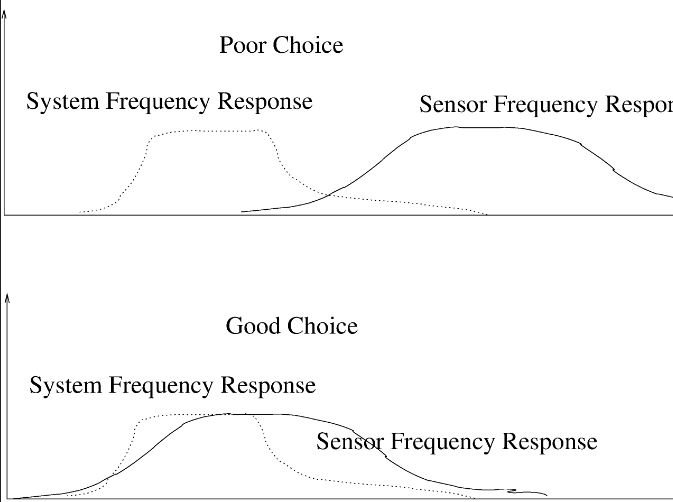
\includegraphics[scale=0.60]{day3_seg1_numerical/sensor_selection.jpg}
\end{frame}

\begin{frame}
  \onslide<1->{
	\frametitle{Kalman Filter Theory vs. Reality} 
	\framesubtitle{}
}
\begin{itemize}
  \onslide<2->{
  \item Choose sensors to match states.\\
E.g., consider the state model
\[
\begin{bmatrix}
\dot{x}_1\\
\dot{x}_2
\end{bmatrix}
= \begin{bmatrix}
0\\
0
\end{bmatrix}
\]
with the measurement model
\[
z = \begin{bmatrix} 1\;\; 0 \end{bmatrix}\begin{bmatrix}
x_1\\
x_2
\end{bmatrix}
+ v
\]
}
  \onslide<3->{
\item   Here $x_1$ is observable but $x_2$ is not, because there are no dynamic paths in $A=I$ flow infomation 
about $x_1$ into $x_2$
}
\end{itemize}
\end{frame}

\begin{frame}
  \onslide<1->{
	\frametitle{Kalman Filter Theory vs. Reality} 
	\framesubtitle{Sensor Selection}
}
\begin{itemize}
  \onslide<2->{
  \item Examine the $H$ matrix that you would use with this sensor!
}
  \onslide<3->{
  \item If it renders some states unobservable, then consider adding 
  additional sensors for those states, or replacing this sensor with one that is more favorable
}
\end{itemize}
\end{frame}
% day3_seg4_ins_challenges/observability.tex
\begin{frame}
  \onslide<1->{
	\frametitle{Observability} 
	\framesubtitle{}
}
\begin{itemize}
  \onslide<2->{
 \item Structural observability is concerned with how $H$ maps measurements into states
}
  \onslide<3->{
  \item Observability means there is a linear path from the measurements to states
}
  \onslide<4->{
  \item Structural observability determined by $\Phi$ and $H$:
}
  \onslide<5->{
\item  If $H$ is $1\times n$, where $n$ is the size of the state vector, then the state $x_0$ 
is said to be \textbf{observable }from $n$ scalar measurements $\set{z_0,\ldots,z_{n-1}}$ if the block matrix
\[
\begin{bmatrix}
H\trans&\Phi\trans H\trans & \cdots & (\Phi\trans)^{n-1}H\trans
\end{bmatrix}
\]
is of rank $n$

}
  \onslide<6->{
 \item Will making measurements as governed by $H$ actually enable us to estimate all of the states 
 in the state vector? 
}
 \end{itemize}
\end{frame}

\begin{frame}
  \onslide<1->{
	\frametitle{Observability} 
	\framesubtitle{Designing Observability into the Filter}
}
\begin{itemize}
  \onslide<2->{
  \item Observability challenge for filters is often a matter of choosing right kinds of sensors
}
  \onslide<3->{
  \item Choosing the right measurement scheduling
}
  \onslide<4->{
  \item Certain kinds of divergence can be the result of poor observability
}
  \onslide<5->{
\item   Example: Let $H=\left[1\;\;0\;\; 0\;\; 0\;\; 0\right]$, 
$\Phi=
\begin{bmatrix}
0&1&0&0&0\\
0&0&1&0&0\\
0&0&0&1&0\\
0&0&0&0&1\\
1& 2&3&4&5
\end{bmatrix}$
}
  \onslide<6->{
	\item What is the rank 
	of $\left[H\trans\;\;\Phi H\trans\;\;\Phi^2 H\trans\;\; \Phi^3 H\trans\;\;\Phi^4 H\trans\right]$?
}
\end{itemize}
\end{frame}



% day2_seg4_numerical/divergence.tex
\begin{frame}
  \onslide<1->{
	\frametitle{Filter Divergence} 
	\framesubtitle{}
}
\begin{itemize}
  \onslide<2->{
\item Kinds of Divergence
}
  \onslide<3->{
\item Causes and Remedies
}
\end{itemize}
\end{frame}

\begin{frame}
  \onslide<1->{
	\frametitle{Filter Divergence} 
	\framesubtitle{Kinds of Divergence}
}
\begin{itemize}
  \onslide<2->{
\item Mean estimation error is supposed to converge to 0
\begin{itemize}
	\item $\esterrdef$
	\item $\expect{\esterr}\rightarrow 0$
	\item Estimate is unbiased: $\expect{\hat{x}(k)}=x(k)$
\end{itemize}
}
  \onslide<3->{
\item Covariance matrix for estimation error is same as state estimation error covariance matrix: $\covmatdef$
}
\end{itemize}
\end{frame}

\begin{frame}
  \onslide<1->{
	\frametitle{Kinds of Divergence} 
	\framesubtitle{}
}
\begin{itemize}
  \onslide<2->{
\item For optimal filter, $P$ will indicate convergence or divergence.
	\begin{itemize}
		\item One common form of divergence due to round-off will send $P$ to zero
	\end{itemize}
}
  \onslide<3->{
\item For suboptimal filters, $P$ will not necessarily indicate divergence
	\begin{itemize}
	  \item $P$ may seem to indicate nominal steady-state values and yet the state estimate may go diverge from the true value
	\end{itemize}
}
\end{itemize}
\end{frame}


\begin{frame}

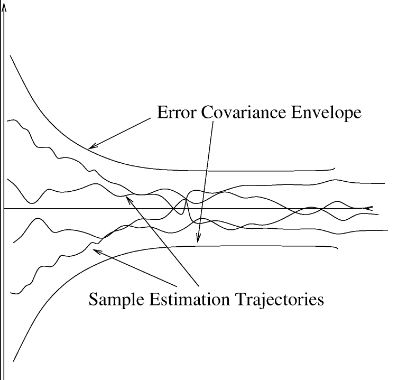
\includegraphics[scale=0.60]{day3_seg1_numerical/covconverge.jpg} 

\end{frame}


\begin{frame}
  \onslide<1->{
	\frametitle{Kinds of Divergence} 
	\framesubtitle{}
}
\begin{itemize}
  \onslide<2->{
\item Going to sleep:  error covariance becomes so small that measurements are no longer believed by the filter
}
  \onslide<3->{
\item Loss of symmetry in $P$
}
  \onslide<4->{
\item Loss of positive definiteness: negative numbers on the diagonal!
}
\end{itemize}
\end{frame}

% day2_seg4_numerical/numstab.tex
\begin{frame}
  \onslide<1->{
	\frametitle{Numerical Stability} 
	\framesubtitle{}
}
\begin{itemize}
  \onslide<2->{
 \item System stability:  Bounded input results in bounded output
}
  \onslide<3->{
 \item Numerical stability: small errors at each computation step do not grow without bound
}
  \onslide<4->{
 \item Matrix Conditioning (will address in discussing SRIF)
}
\end{itemize}
\end{frame}

%\input{day2_seg4_numerical/matrix_conditioning.tex}
% day2_seg4_numerical/roundoff.tex
\begin{frame}
  \onslide<1->{
	\frametitle{Round-Off Errors} 
	\framesubtitle{Joseph Form}
}
\begin{itemize}
  \onslide<2->{
 \item Computer round-off in floating point arithmetic
}
  \onslide<3->{
 \item Unit round-off value is largest number $\eps$ such that $1+\eps=1$
}
  \onslide<4->{
 \item In Matlab, the global symbol "eps" stores the unit round-off value
}
  \onslide<5->{
  \item Round-off errors generally plague the classical covariance update algorithm
\[\covupdateeq\]
\begin{itemize}
  \item Alternative, called the Joseph form, is more robust:
\[\josephcovupdateeq\]
\end{itemize} 
}
\end{itemize}
\end{frame}

\begin{frame}
  \onslide<1->{
	\frametitle{Round-Off Errors} 
	\framesubtitle{De Vries Mechanization}
}
\begin{itemize}
  \onslide<2->{
\item   This form in turn leads to the De Vries mechanization of the
Kalman gain equation.  To see this, first expand
the Joseph form (omitting subscripts for clarity):

}
  \onslide<3->{
\begin{align*}
   P(+)&= P(-)-KHP(-)-P(-)H\trans K\trans+ KHP(-)H\trans K\trans +
   KRK\trans.
\end{align*}
}
\end{itemize}
\end{frame}

\begin{frame}
  \onslide<1->{
	\frametitle{Round-Off} 
	\framesubtitle{De Vries}
}
\begin{itemize}
  \onslide<2->{
\item   Define
\begin{equation}\label{Feq}
  F=PH\trans
\end{equation}
and
\begin{equation}\label{Deq}
  D=HF+R.
\end{equation}

}
  \onslide<3->{
\item   We note that $D$ is symmetric, because
\begin{align*}
  D\trans &= [HF+R]\trans \\
  &= [HPH\trans + R]\trans \\
  &= [HPH\trans] \trans + R\trans \\
  &= [H\trans]\trans P\trans H\trans + R\trans \\
  &= HPH\trans + R & \text{(because $P$ and $R$ are symmetric)}\\
  &= HF + R \\
  &= D.
\end{align*}
}
\end{itemize}
\end{frame}

\begin{frame}
  \onslide<1->{
	\frametitle{Round-Off} 
	\framesubtitle{De Vries}
}
\begin{itemize}
  \onslide<2->{
\item   The gain in standard Kalman gain equation
\[\kalgaineq\] can be written as
\[K=FD^{-1}.\]
}
  \onslide<3->{
\item   Using Eqs.~(\ref{Feq}) and ~(\ref{Deq}), we compute
\begin{align*}
  P(+) &= P(-) - KF\trans - FK\trans + KDK\trans \\
  &= P(-)-K\left[F\trans - \frac{DK\trans}{2} \right] - \left[
  F-\frac{KD}{2}\right]K\trans.
\end{align*}

}
  \onslide<4->{
\item   Letting $G=F-\dfrac{KD}{2}$, we obtain
\begin{equation}\label{dvcovupdateeq}
  \dvcovupdateeq.
\end{equation}

}
\end{itemize}
\end{frame}

\begin{frame}
  \onslide<1->{
	\frametitle{Round-Off} 
	\framesubtitle{De Vries}
}
\begin{itemize}
  \onslide<2->{
\item   The De Vries mechanization implements Eq.~(\ref{dvcovupdateeq}) by
subtracting the $ij^{th}$ element of $GK\trans$ from both the
$ij^{th}$ and $ji^{th}$ elements of $P(-)$. 
}
  \onslide<3->{
\item   The De Vries form of
the covariance update equation is valid for any arbitrary gain
matrix $K$, not just the optimal gains computed from
Eqs.~(\ref{Feq}) and (\ref{Deq}).

}
\end{itemize}
\end{frame}

% day2_seg4_numerical/matinv.tex
\begin{frame}
  \onslide<1->{
	\frametitle{Numerical Stability} 
	\framesubtitle{Matrix Inversion}
}
\begin{itemize}
  \onslide<2->{
 \item Matrix inversion is always risky due to potential ill-conditioning
}
  \onslide<3->{
 \item One way to avoid this is to process measurements sequentially as scalars
}
  \onslide<4->{
 \item Or at least as low-dimensional matrices
}
\end{itemize}
\end{frame}

%% day2_seg4_numerical/symmloss.tex
\begin{frame}
Loss of Symmetry and Positive Definiteness
 \begin{itemize}
 \item
 \item
 \item
\end{itemize}
\end{frame}

% day2_seg4_numerical/exercises.tex
\begin{frame}
  \onslide<1->{
	\frametitle{Exercises} 
}
\begin{itemize}
  \onslide<2->{
\item   1. Let $v=[1\;\; -2]\trans$.  Compute the positive definite, symmetrix matrix $M=vv\trans$

}
  \onslide<3->{
\item   2. Use the following algorithm (Grewal \& Andrews) to factor $M$ into $UDU\trans$ form:
}
\end{itemize}
\end{frame}
\begin{frame}[fragile]
	\frametitle{Exercises} 
\begin{verbatim}
for j=m:-1:1
    for i=j:-1:1
        covar=P(i,j);
        for k=j+1:m
            covar=covar-U(i,k)*D(k,k)*U(j,k);
        end
        if i==j
            D(j,j)=covar;
            U(j,j)=1;
        else
            U(i,j)=covar/D(j,j);
        end
    end
end
\end{verbatim}
\end{frame}

